\documentclass{beamer}

\usetheme{Madrid}

\usepackage{graphicx} % Allows including images
\graphicspath{{./../img/}}

\title{Theia Status Update and Tutorial}

\author{Optics Group, Virgo}
\date{Wednesday, June 28\textsuperscript{th} 2017} % Date, can be changed to a custom date

\begin{document}

\begin{frame}
\titlepage % Print the title page as the first slide
\end{frame}




%------------------------------------------------

\begin{frame}
\frametitle{Reminder}

\texttt{theia}:

\begin{itemize}
\item General astigmatic beam tracer in 3D
\item With support for many optical components(mirrors, thin lenses, thick lenses, beamdumps)
\item And many Gaussian functions

\item Reading and writing standard input (\texttt{.tia}) and output (\texttt{.out}) text files
\item And with 3D visualization capabilities by exporting to CAD software

\item Geometric optics: no approximation
\item Soon: cavities, interferences
\end{itemize}
\end{frame}

\begin{frame}
\frametitle{News}

\begin{itemize}
\item June 9\textsuperscript{th}: \texttt{theia 0.1.0}
\item Idea: Virgo Hub on \texttt{hub.virgo-gw.eu} for home-made software (\texttt{theia}, \texttt{BruCo}, etc.) ? $\rightarrow$ Question pending...
\item In the mean time: sources, documentation, news on \url{http://theia.hopto.org:56000}

\item And: Internship presentation (July 7\textsuperscript{th}), Virgo Week ($\sim$July 15\textsuperscript{th})
\end{itemize}
\end{frame}


\begin{frame}
\frametitle{Before (May 10\textsuperscript{th}) ...}
\begin{figure}
\begin{center}
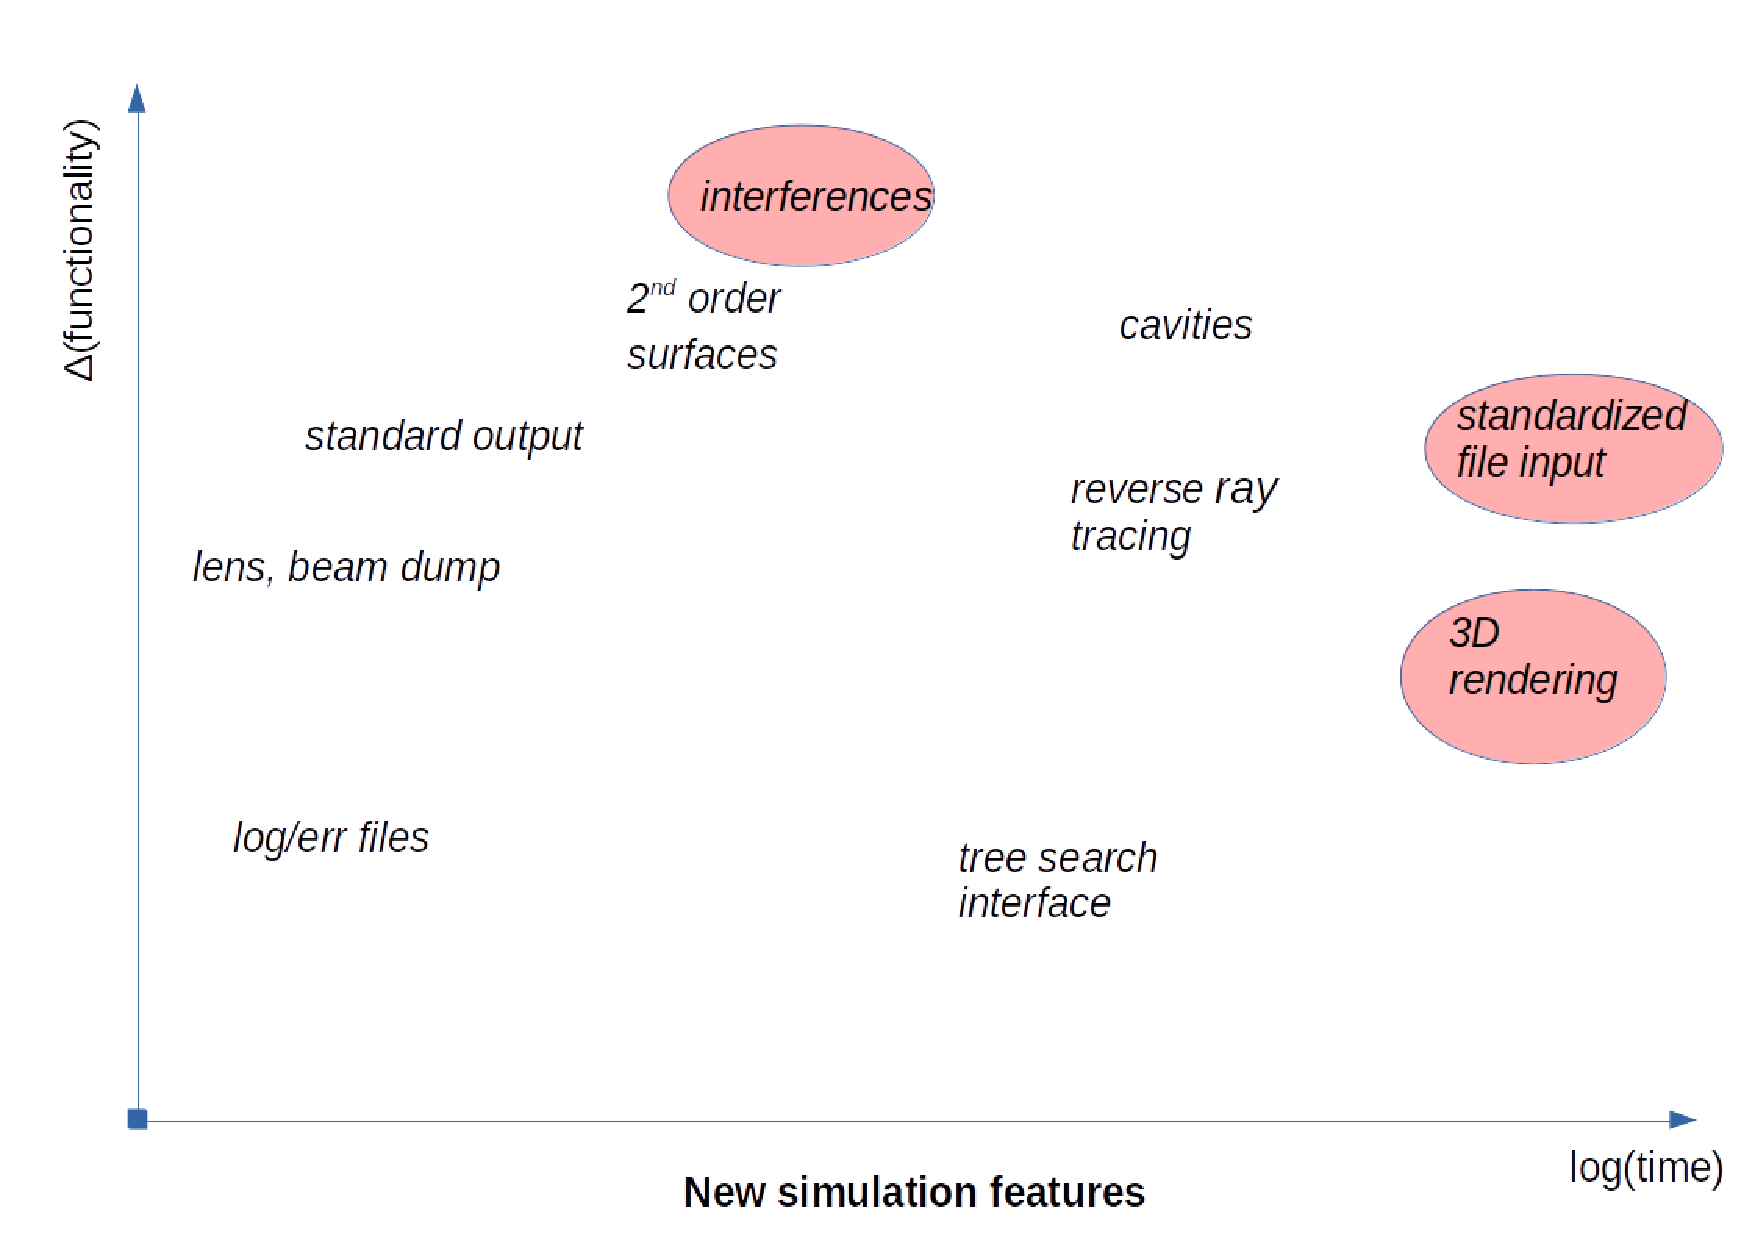
\includegraphics[scale=0.36]{newfeatures.pdf}
\end{center}
\end{figure}
\end{frame}

\begin{frame}
\frametitle{... After (June 28\textsuperscript{th})}
\begin{figure}
\begin{center}
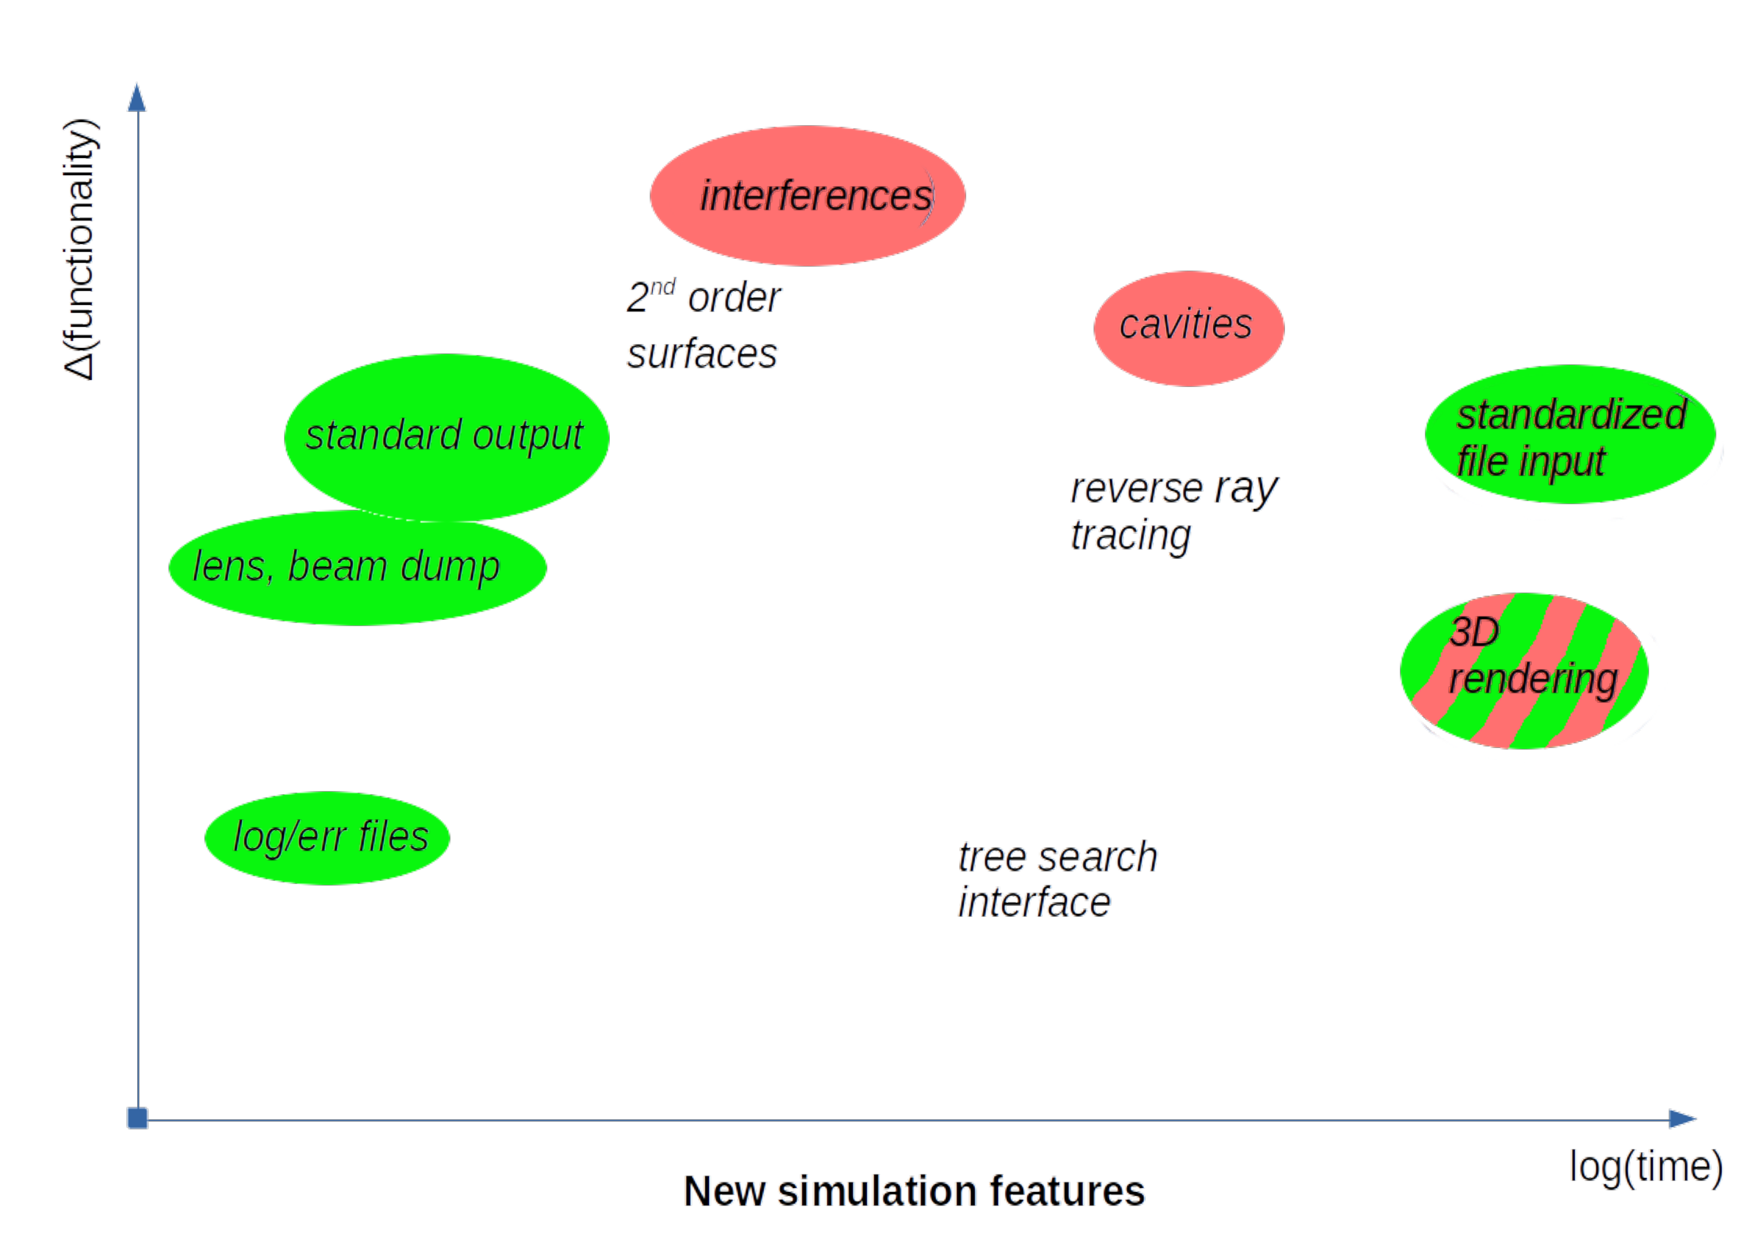
\includegraphics[scale=0.36]{newfeatures2.pdf}
\end{center}
\end{figure}
\end{frame}

\begin{frame}
\frametitle{Quick Tour}

\url{http://theia.hopto.org:56000}
\end{frame}


\begin{frame}
\frametitle{Tutorial: CLI tool }
\begin{itemize}
\item \texttt{theia} CLI tool
\item \texttt{theia} as a library
\end{itemize}
\end{frame}

\begin{frame}
\frametitle{Tutorial: Library tool }
\begin{center}
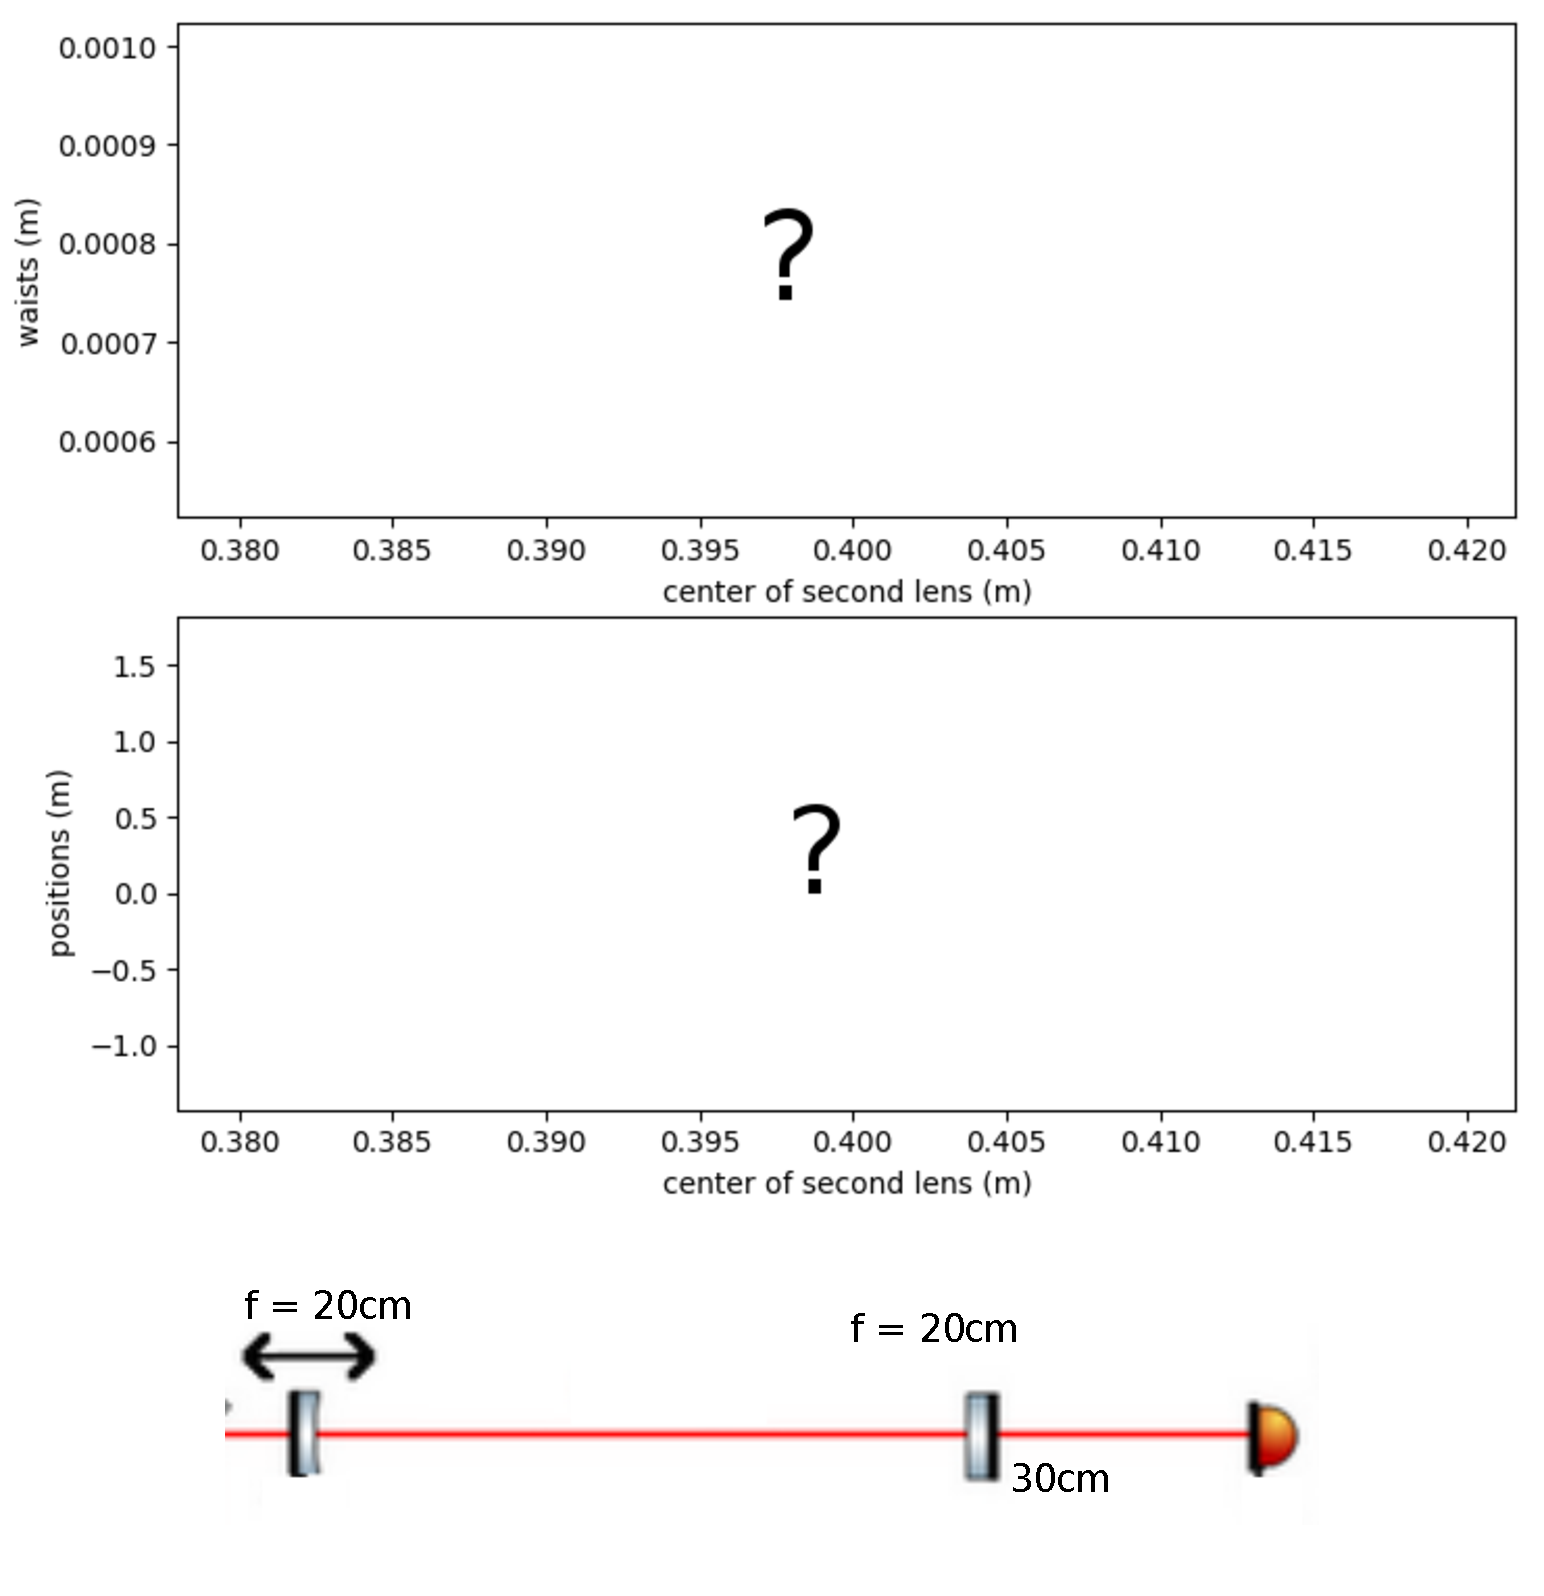
\includegraphics[scale=.3]{emptygraph.pdf}
\end{center}



\end{frame}
\end{document} 
